\documentclass{article}
    
    \usepackage{graphicx} % Used to insert images
    \usepackage{adjustbox} % Used to constrain images to a maximum size 
    \usepackage{color} % Allow colors to be defined
    \usepackage{enumerate} % Needed for markdown enumerations to work
    \usepackage{geometry} % Used to adjust the document margins
    \usepackage{amsmath} % Equations
    \usepackage{amssymb} % Equations
    \usepackage{eurosym} % defines \euro
    \usepackage[mathletters]{ucs} % Extended unicode (utf-8) support
    \usepackage[utf8x]{inputenc} % Allow utf-8 characters in the tex document
    \usepackage{fancyvrb} % verbatim replacement that allows latex
    \usepackage{grffile} % extends the file name processing of package graphics 
                         % to support a larger range 
    % The hyperref package gives us a pdf with properly built
    % internal navigation ('pdf bookmarks' for the table of contents,
    % internal cross-reference links, web links for URLs, etc.)
    \usepackage{hyperref}
    \usepackage{longtable} % longtable support required by pandoc >1.10
    \usepackage{booktabs}  % table support for pandoc > 1.12.2
    \usepackage{indentfirst}
    \usepackage{floatrow}
    \usepackage{relsize}
        
    \newcommand\perm[2]{{}_{#1}P_{#2}}%
    \newcommand\todo[1]{\textbf{TODO: #1}}% 
    \newcommand\numberthis{\addtocounter{equation}{1}\tag{\theequation}}
    \newcommand\seteq{\mathrel{\overset{\makebox[0pt]{\mbox{\normalfont\small\sffamily set}}}{=}}}
    \newcommand\mfrac[2]{\left(\dfrac{#1}{#2}\right)}
    
    \title{Homework 10}
    \author{Roly Vicar\'ia \\ STAT414 Spring 2016}
    
\begin{document}
    
    \maketitle
    
    \textbf{Section 4.1}
    \begin{enumerate}
     %1
     \item 
      \begin{enumerate}
       %a
       \item 
	\begin{align*}
	  \mathlarger{\sum}_{x=1}^2 \mathlarger{\sum}_{y=1}^3 {c(x+2y)} 
	    &= c(1+2(1)) + c(1+2(2)) + c(1+2(3)) + c(2+2(1)) + c(2+2(2)) + c(2+2(3)) \\
	    &= 33c \seteq 1
	\end{align*}
	Therefore, $c=\dfrac{1}{33}$
       
       %b
       \item
	\begin{align*}
	 \mathlarger{\sum}_{x=1}^3 \mathlarger{\sum}_{y=1}^x {c(x+y)}
	  &= c(1+1) + c(2+1) + c(2+2) + c(3+1) + c(3+2) + c(3+3) \\
	  &= 24c \seteq 1
	\end{align*}
	Therefore, $c = \dfrac{1}{24}$
       
       %c
       \item
	\begin{align*}
	 \mathlarger{\sum}_{y=0}^5 \mathlarger{\sum}_{x=6-y}^{8-y} {c}
	  &= 18c \seteq 1
	\end{align*}
	Therefore, $c = \dfrac{1}{18}$
       
       %d
       \item
	\begin{align*}
	 \mathlarger{\sum}_{x=1}^\infty \mathlarger{\sum}_{y=1}^\infty 
	    {c\mfrac{1}{4}^x\mfrac{1}{3}^y}
	  &= \mathlarger{\sum}_{x=1}^\infty \left\{c\mfrac{1}{4}^x 
	      \left[\mfrac{1}{3}^1 + \mfrac{1}{3}^2 + \cdots \right] \right\} \\
	  &= \mathlarger{\sum}_{x=1}^\infty \left\{c\mfrac{1}{4}^x 
	      \left[\dfrac{1/3}{1 - 1/3}\right] \right\} \\
	  &= \mathlarger{\sum}_{x=1}^\infty {\dfrac{c}{2}\mfrac{1}{4}^x} \\
	  &= \dfrac{c}{2}\left[\mfrac{1}{4}^1 + \mfrac{1}{4}^2 + \cdots \right] \\
	  &= \dfrac{c}{2} \left[ \dfrac{1/4}{1 - 1/4} \right] \\
	  &= \dfrac{c}{6} \seteq 1
	\end{align*}
	Therefore, $c = 6$.
      \end{enumerate}     
     \addtocounter{enumi}{1}
      
     %3
     \item
      \begin{enumerate}
       %a
       \item 
	$f_x(x) = \mathlarger{\sum}_{y=1}^4{\dfrac{x+y}{32} = \dfrac{x+1}{32} + \dfrac{x+2}{32}
	  +\dfrac{x+3}{32} + \dfrac{x+4}{32}} = \dfrac{4x+10}{32} = \dfrac{2x+5}{16}, x=1,2$
       
       %b
       \item 
	$f_y(y) = \mathlarger{\sum}_{x=1}^2{\dfrac{x+y}{32}} = \dfrac{1+y}{32} + \dfrac{2+y}{32}
	  = \dfrac{3+2y}{32}, y=1,2,3,4$
       
       %c
       \item 
	$P(X > Y) = f(2,1) = \dfrac{2+1}{32} = \dfrac{3}{32}$
       
       %d
       \item 
	$P(Y = 2X) = f(1,2) + f(2,4) = \dfrac{1+2}{32} + \dfrac{2+4}{32} = \dfrac{9}{32}$
       
       %e
       \item 
	$P(X + Y = 3) = f(1,2) + f(2,1) = \dfrac{1+2}{32} + \dfrac{2+1}{32} = \dfrac{6}{32} = \dfrac{3}{16}$
       
       %f
       \item 
	$P(X \le 3 - Y) = P(X + Y \le 3) = f(1,1) + f(1,2) + f(2,1) = \dfrac{1+1}{32} + \dfrac{1+2}{32}
	  + \dfrac{2+1}{32} = \dfrac{8}{32} = \dfrac{1}{4}$
       
       %g
       \item 
	$f(1,3) = \dfrac{1+3}{32} = \dfrac{1}{8} \neq f_x(1)f_y(3) 
	      = \mfrac{7}{16}\mfrac{9}{32} = \dfrac{63}{512}$
       
       %h
       \item 
	\begin{align*}
	 \mu_x &= \mathlarger{\sum}_{x=1}^2 \mathlarger{\sum}_{y=1}^4 {x\mfrac{x+y}{32}} \\
	  &= 1\left[\dfrac{1+1}{32} + \dfrac{1+2}{32} + \dfrac{1+3}{32} + \dfrac{1+4}{32}\right]
	    + 2\left[\dfrac{2+1}{32} + \dfrac{2+2}{32} + \dfrac{2+3}{32} + \dfrac{2+4}{32}\right] \\
	  &= \dfrac{14}{32} + \dfrac{36}{32} \\
	  &= \dfrac{25}{16} = 1.5625 
	\end{align*}
	
	\begin{align*}
	 \sigma_x^2 &= \mathlarger{\sum}_{x=1}^2 \mathlarger{\sum}_{y=1}^4 
	      {\left(x-\dfrac{25}{16}\right)^2\mfrac{x+y}{32}} \\
	  &= \left(1-\dfrac{25}{16}\right)^2 \left[\dfrac{1+1}{32} + \dfrac{1+2}{32} + \dfrac{1+3}{32} + \dfrac{1+4}{32}\right]
	    + \left(2-\dfrac{25}{16}\right)^2\left[\dfrac{2+1}{32} + \dfrac{2+2}{32} + \dfrac{2+3}{32} + \dfrac{2+4}{32}\right] \\
	  &= \dfrac{81}{256}\mfrac{14}{32} + \dfrac{49}{256}\mfrac{18}{32} \\
	  &= \dfrac{63}{256} \approx 0.2461 
	\end{align*}
	\begin{align*}
	 \mu_y &= \mathlarger{\sum}_{y=1}^4 \mathlarger{\sum}_{x=1}^2 {y\mfrac{x+y}{32}} \\
	  &= 1\left[\dfrac{1+1}{32} + \dfrac{2+1}{32}\right] + 2\left[\dfrac{1+2}{32} + \dfrac{2+2}{32}\right]
	    + 3\left[\dfrac{1+3}{32} + \dfrac{2+3}{32}\right] + 4\left[\dfrac{1+4}{32} + \dfrac{2+4}{32}\right] \\
	  &= \dfrac{5}{32} + \dfrac{14}{32} + \dfrac{27}{32} + \dfrac{44}{32} \\
	  &= \dfrac{90}{32} = \dfrac{45}{16} = 2.8125 
	\end{align*}
	\begin{align*}
	 \sigma_y^2 &= \mathlarger{\sum}_{y=1}^4 \mathlarger{\sum}_{x=1}^2
	      {\left(y-\dfrac{45}{16}\right)^2\mfrac{x+y}{32}} \\
	  &= \left(1-\dfrac{45}{16}\right)^2\left[\dfrac{1+1}{32} + \dfrac{2+1}{32}\right] 
	    + \left(2-\dfrac{45}{16}\right)^2\left[\dfrac{1+2}{32} + \dfrac{2+2}{32}\right]
	    + \left(3-\dfrac{45}{16}\right)^2\left[\dfrac{1+3}{32} + \dfrac{2+3}{32}\right] \\
	  &\mspace{20mu}+ \left(4-\dfrac{45}{16}\right)^2\left[\dfrac{1+4}{32} + \dfrac{2+4}{32}\right] \\
	  &= \dfrac{841}{256}\mfrac{5}{32} + \dfrac{169}{256}\mfrac{7}{32}
	    + \dfrac{9}{256}\mfrac{9}{32} + \dfrac{361}{256}\mfrac{11}{32} \\
	  &= \dfrac{295}{256} \approx 1.1523
	\end{align*}
      \end{enumerate}
     \addtocounter{enumi}{4}
     
     %8
     \item
      \begin{enumerate}
       %a
       \item
	$f(x,y) = \dfrac{7!}{x!y!(7-x-y)!}(0.78)^{x}(0.01)^{y}(0.21)^{7-x-y}, x+y \le 7$
       
       %b
       \item
	$f_x(x) = \dfrac{7!}{x!(7-x)!}(0.78)^x(0.22)^{7-x}, x \le 7$
      \end{enumerate}
      
     %9
     \item
      \begin{enumerate}
       %a
       \item 
	$f(x,y) = \mfrac{15!}{x!y!(15-x-y)!}\mfrac{6}{10}^x\mfrac{3}{10}^y\mfrac{1}{10}^{15-x-y}
	  , 0 \le x+y \le 15$
       
       %b
       \item
	Based on the shape of the region, they cannot be independent because the region is not
	rectangular.
	
	\begin{figure}[h!]
	  \centering
	  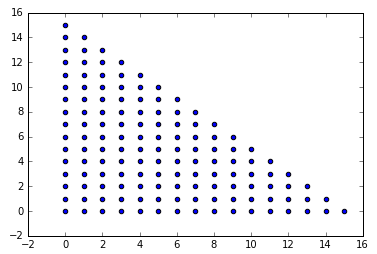
\includegraphics[scale=.6,keepaspectratio=true]{./images/scatterPlot_XandY_lessThanEq_15.png}
	  % scatterPlot_XandY_lessThanEq_15.png: 377x254 pixel, 96dpi, 9.97x6.72 cm, bb=0 0 283 190
	\end{figure}
       
       %c
       \item
	$f(10,4) = \mfrac{15!}{10!4!1!}\mfrac{6}{10}^{10}\mfrac{3}{10}^4\mfrac{1}{10}^1
	  \approx 0.07354$
       
       %d
       \item
	$X \sim b(15, 0.6)$
       
       %e
       \item
	\begin{align*}
	  P(X \le 11) &= 1 - P(X > 11) \\
	    &= 1 - [P(X = 12) + P(X = 13) + P(X = 14) + P(X = 15)] \\
	    &= 1 - \left[\dfrac{15!}{12!3!}(.6)^{12}(.4)^3 + \dfrac{15!}{13!2!}(.6)^{13}(.4)^2
	      + \dfrac{15!}{14!1!}(.6)^{14}(.4)^{1} + \dfrac{15!}{15!0!}(.6)^{15}(.4)^0 \right] \\
	    &= 1 - 0.0905 \\
	    &= 0.9095
	\end{align*}	
      \end{enumerate}
    \end{enumerate}
    
    \newpage
    \textbf{Section 4.2}
    \begin{enumerate}
     %1
     \item
      \begin{align*}
	 \mu_x &= \mathlarger{\sum}_{x=1}^2 \mathlarger{\sum}_{y=1}^4 {x\mfrac{x+y}{32}} 
	  = \dfrac{25}{16} = 1.5625 \\
	  \\
	 \sigma_x^2 &= \mathlarger{\sum}_{x=1}^2 \mathlarger{\sum}_{y=1}^4 
	      {\left(x-\dfrac{25}{16}\right)^2\mfrac{x+y}{32}}   
	  = \dfrac{63}{256} \approx 0.2461 \\
	  \\
	 \mu_y &= \mathlarger{\sum}_{y=1}^4 \mathlarger{\sum}_{x=1}^2 {y\mfrac{x+y}{32}} 
	  = \dfrac{90}{32} = \dfrac{45}{16} = 2.8125 \\
	  \\
	 \sigma_y^2 &= \mathlarger{\sum}_{y=1}^4 \mathlarger{\sum}_{x=1}^2
	      {\left(y-\dfrac{45}{16}\right)^2\left(\dfrac{x+y}{32}\right)}
	  = \dfrac{295}{256} \approx 1.1523 \\
	  \\
	 Cov(X,Y) &= \left[\mathlarger{\sum}_{x=1}^2 \mathlarger{\sum}_{y=1}^4 {xy \dfrac{x+y}{32}}\right] 
		- \mfrac{25}{16}\mfrac{45}{16} \\
	    &= (1)(1)\dfrac{2}{32} + (1)(2)\dfrac{3}{32} + (1)(3)\dfrac{4}{32} + (1)(4)\dfrac{5}{32} \\
	     &\mspace{40mu}+ (2)(1)\dfrac{3}{32} + (2)(2)\dfrac{4}{32} + (2)(3)\dfrac{5}{32} 
		+ (2)(4)\dfrac{6}{32} - \dfrac{1125}{256}\\
	    &= -\dfrac{5}{256} \approx -0.01953 \\
	  \\
	 \rho &= \dfrac{Cov(X,Y)}{\sigma_x\sigma_y} 
	    = \dfrac{-\dfrac{5}{256}}{\sqrt{\dfrac{63}{256}\cdot\dfrac{295}{256}}}
	    \approx -0.03668
      \end{align*}
     \addtocounter{enumi}{2}
     
     \newpage
     %4
     \item
      \begin{enumerate}
       %a
       \item $E(X) = np_x = 3\mfrac{1}{6} = \dfrac{1}{2}$
       
       %b
       \item $E(Y) = np_y = 3\mfrac{1}{2} = \dfrac{3}{2}$
       
       %c
       \item 
	$Var(X) = np_x(1-p_x) = 3\mfrac{1}{6}\mfrac{5}{6} = \dfrac{5}{12}$
       
       %d
       \item
	$Var(Y) = np_y(1-p_y) = 3\mfrac{1}{2}\mfrac{1}{2} = \dfrac{3}{4}$
       
       %e
       \item $Cov(X,Y) = \rho \sigma_x \sigma_y 
	  = -\sqrt{\mfrac{1}{5}\mfrac{5}{12}\mfrac{3}{4}} = -\dfrac{1}{4}$
       
       %f
       \item
	$\rho = -\sqrt{\dfrac{p_x p_y}{(1-p_x)(1-p_y)}} 
	  = -\sqrt{\dfrac{\mfrac{1}{6}\mfrac{1}{2}}{\mfrac{5}{6}\mfrac{1}{2}}}
	  = -\sqrt{\dfrac{1}{5}}$
      \end{enumerate}
     
     %5
     \item
      We begin by expanding the expression in the expectation,
      \begin{align*}
       K(a,b) &= E[(Y - a - bX)^2] \\
	&= E[Y^2 - 2aY - 2bXY + a^2 + 2abX + b^2X^2] \\
	&= E(Y^2) - 2aE(Y) - 2bE(XY) + a^2 + 2abE(X) + b^2E(X^2) \\
	&= E(Y^2) - \mu_y^2 + \mu_y^2 - 2a\mu_y - 2bE(XY) + a^2
	  + 2ab\mu_x + b^2E(X^2) - b^2\mu_x^2 + b^2\mu_x^2 \\
	&= a^2 - 2a\mu_y - 2b(\mu_x\mu_y + \sigma_{xy}) + 2ab\mu_x + b^2(\sigma_x^2 
	  + \mu_x^2) + \sigma_y^2 + \mu_y^2
      \end{align*}

      Now we will compute the partial derivatives of that expression with respect to $a$ and $b$,
      \begin{align*}
       \dfrac{\partial K}{\partial a} &= 2a -2\mu_y + 2b\mu_x \\
       \\
       \dfrac{\partial K}{\partial b} &= -2(\mu_x\mu_y + \sigma_{xy}) + 2a\mu_x
	  + 2b(\sigma_x^2 + \mu_x^2)
      \end{align*}

      Setting the first of these equal to 0,
      \begin{align*}
       2a - 2\mu_y + 2b\mu_x &\seteq 0 \\
       a - \mu_y + b\mu_x &= 0 \\
       a &= \mu_y - b\mu_x
      \end{align*}

      We then substitute this for $a$ in the second partial derivative and set equal to 0,
      \begin{align*}
       -2(\mu_x\mu_y + \sigma_{xy}) + 2(\mu_y - b\mu_x)\mu_x + 2b(\sigma_x^2 + \mu_x^2) &\seteq 0 \\
       -\mu_x\mu_y - \sigma_{xy} + \mu_x\mu_y - b\mu_x^2 + b\sigma_x^2 + b\mu_x^2 &= 0 \\
       b &= \dfrac{\sigma_{xy}}{\sigma_x^2}
      \end{align*}
      
      Therefore, the line found by method of least squares is,
      \begin{align*}
       y = \mu_y - \mu_x\mfrac{\sigma_{xy}}{\sigma_x^2} + \mfrac{\sigma_{xy}}{\sigma_x^2}x
      \end{align*}
     \addtocounter{enumi}{1}
     
     %7
     \item
      \begin{enumerate}
       %a
       \item
	X and Y are dependent because the joint probability is not ``rectangular''
       
       %b
       \item
	\begin{align*}
	  Cov(X,Y) &= E(XY) - \mu_x\mu_y \\
	    &= (0)(0)\mfrac{1}{4} + (1)(1)\mfrac{1}{4} + (1)(-1)\mfrac{1}{4} + (2)(0)\mfrac{1}{4} 
	      - (1)(0) \\ 
	    &= 0 \\
	    \\
	  \rho &= \dfrac{Cov(X,Y)}{\sigma_x \sigma_y} = 0
	\end{align*}
      \end{enumerate}
    \end{enumerate}

\end{document}